\section{Oscillation Theory and the PMNS Matrix}

In 1957, Bruno Pontecorvo suggested a possible mechanism for the transition between exotic atoms known as muonium and the corresponding anti-atom, anti-muonium \cite{Pontecorvo-Mesonium}.
Pontecorvo noted that this transition would not be disallowed if proceeding via the conversion of the muon ane electron into the one neutrino flavor then-known.

\begin{equation}
   \left(\mu^+ e^-\right) \rightarrow \nu + \bar{\nu} \rightarrow \left(\mu^- e^+\right)
\end{equation}

At the time, the muon neutrino was not yet known as a separate particle, a discovery not made until 1962 \cite{Danby-NuMu}.
Pontecorvo noted that this process would be rather slow, with a rate $\mathtt{10^{10}}$ times slower than the typical muon decay. 
If, however, the muonium and anti-munium possessed different masses and could interact directly, the mixing between the states could proceed significantly faster with a rate only 300 times slower than muon decays.

While there is not known direct mixing between the muonium and anti-muonium atoms, Pontecorvo's work laid the groundwork for understanding the process of \emph{neutrino oscillations}, a process to which it was applied by Pontecorvo himself in 1968 \cite{Pontecorvo-Oscillations}.
The process was further developed for the neutrino sector by Ziro Maki, Masami Nakagawa and Shoichi Sakata in 1962 \cite{Maki-Nakagawa-Sakata}.

\subsection{The PMNS Mixing Matrix}

We now understand there to be three distinct flavors of neutrinos.
Specifically, there exist three weak eigenstates of the left-handed neutrino fields that are related to three known neutrino mass eigenstates via the lepton mixing matrix known as the \emph{PMNS} (Pontecorvo-Maki-Nakagawa-Sakata).

\begin{equation}
\begin{pmatrix} \nu_e\left(x\right) \\ 	\nu_\mu\left(x\right) \\	\nu_\tau\left(x\right) \end{pmatrix} = 
U_{PMNS} \begin{pmatrix} \nu_e\left(x\right) \\ 	\nu_\mu\left(x\right) \\	\nu_\tau\left(x\right) \end{pmatrix} = 
\begin{pmatrix}
 U_{e 1} & U_{e 2} & U_{e 3} \\
 U_{\mu 1} & U_{\mu 2} & U_{\mu 3} \\
 U_{\tau 1} & U_{\tau 2} & U_{\tau 3} \\
\end{pmatrix} 	
\begin{pmatrix} \nu_1\left(x\right) \\ 	\nu_2\left(x\right) \\	\nu_3\left(x\right) \end{pmatrix}
\label{eqn:3flavor_pmns}
\end{equation}

The flavor eigenstates ($\mathtt{\nu_e}$, $\mathtt{\nu_\mu}$, $\mathtt{\nu_\tau}$) describe the fields of the left-handed neutrinos coupling via the weak charge to the electron, muon, and tau respectively.
The three mass states ($\mathtt{\nu_1}$, $\mathtt{\nu_2}$, $\mathtt{\nu_3}$) represent the mass eigenstates.
The mixing between the two types of states is given by the unitary matrix, $U_{PMNS}$.
In general, the mixing may be written in a shortened form

\begin{equation}
\nu_{\alpha}\left(x\right) = \sum_i U_{\alpha i} \nu_{i}\left(x\right)
\label{eqn:3flavor_short}
\end{equation}

where $\mathtt{\alpha=e,\mu,\tau}$ and $\mathtt{i=1,2,3}$. 

Neutrinos interact solely via the weak force and are therefore created in these states.
The neutrino produced in state $\nu_\alpha$, therefore, exists in a superposition of the three mass eigenstates.

where $\mathtt{\delta_{ij}}$ is the Kronecker delta function.
As a 3 $\mathtt{\times}$ 3 unitary matrix, the PMNS matrix may be parametrized in terms of three mixing angles and six phases.
Of these phases, five may be removed by rephasing the lepton fields with no change to the underlying physics, leaving one physical phase ralted to CP violation.

The PMNS may be written in terms of the product of three smaller unitary matrices using these mixing angles.

\begin{equation}
U_{PMNS} = 
\begin{pmatrix}
1 & 0 & 0 \\
0 & c_{23} & s_{23} \\
0 & -s_{23} & c_{23} \\
\end{pmatrix}
\begin{pmatrix}
c_{13} & 0 & s_{13} e^{-i\delta_{CP}} \\
0 & 1 & 0 \\
-s_{13} e^{i \delta_{CP}} & 0 & c_{13} \\
\end{pmatrix}
\begin{pmatrix}
c_{12} & s_{12} & 0 \\
-s_{12} & c_{12} & 0 \\
0 & 0 & 1 \\
\end{pmatrix}
\label{eqn:pmns_parametrized}
\end{equation}

where the notation $\mathtt{c_{ij}}$ is used to denote $\mathtt{\cos\left(\theta_{ij}\right)}$ and $\mathtt{s_{ij}}$ is used for $\mathtt{\sin\left(\theta_{ij}\right)}$.

Note that if neutrinos are Majorana fermions, the additional phases may not be removed without making the masses complex.
The Majorana terms form additional diagonal terms in Equation~\ref{eqn:pmns_parametrized}.
While Majorana mass terms are beyond the scope of this work, further information may be found in \cite{Review-PMNS,Review-MajoranaNu}.

The three submatrices of Equation~\ref{eqn:pmns_parametrized} have historically been studied by different types of experiments. 
This history has lead to the proliferation of alternative names for the matrices and, therefore, of the mixing angles.

\begin{equation}
U_{PMNS} = U_{Atmospheric} U_{Reactor} U_{Solar}
\end{equation}

This leads to the alternative names of the mixing angles, with $\mathtt{\theta_{23}}$, $\mathtt{\theta_{13}}$, and $\mathtt{\theta_{12}}$ being referred to as the atmospheric mixing angle, the reactor mixing angle, and the solar mixing angle respectively.

\label{subsec:vacuum}
\subsection{Neutrino Mixing in Vacuum}
Neutrinos are created via the weak force as pure flavor eigenstates. 
These states are coherent superpositions of mass eigenstates described by Equation~\ref{eqn:3flavor_short}.

\begin{equation}
\ket{\nu\left(t=0\right)} = \ket{\nu_\alpha} = \sum_i U_{\alpha i}^* \ket{\nu_i}
\end{equation}

The flavor states are not eigenstates of the Hamiltonian, however.
For propagation of the neutrino, the mass eigenstates must instead be used.
The propagation leads to a neutrino state at time $\mathtt{t}$ which is no longer a pure flavor state

\begin{equation}
\ket{\nu\left(t\right)} = \sum_i U^*_{\alpha i} e^{-iE_i t} \ket{\nu_i}
\end{equation}
\begin{equation}
\ket{\nu\left(t\right)} = \sum_i U^*_{\alpha i} e^{-iE_i t} \sum_{\beta} U_{\beta i} \ket{\nu_\beta}
\end{equation}

where $\mathtt{E_i} = \sqrt{p^2+m_i^2}$ is the total energy of the $\mathtt{i}$th mass eigenstate.
If the neutrino state interacts again, the flavor eigenstate must again be used to calculate the probabilities of interacting as each of the three known flavors.

\begin{equation}
P\left(\nu_\alpha\rightarrow\nu_\beta\right) = \left|\bra{\nu_\beta}\ket{\nu\left(t\right)}\right|^2 
                 															= \left|\sum_i U_{\beta i} U^*_{\alpha i} e^{-i E_i t} \right|^2
\label{eqn:pmns_probability}
\end{equation}

Proper calculations from this point can be performed by treating each neturino as a quantum mechanical wave packet \cite{OscillationWavePackets}.
This allows for the full description of neutrino oscillation in the context of decoherence of the mass states during propagation, allowing each mass state to possess separate momenta.

In practice, the description of neutrino oscillations necessary for this work is adequately described by making a few simplifying assumptions.
In particular, this work assumes that all mass eigenstates propagate as plane waves possessing identical, well-defined momenta \cite{Review-PMNS}.
Neutrinos are further assumed to be extremely relativistic at the energies of interest, an assumption well-justified by cosmological fits to the sum of the three neutrino masses, which give an upper limit of around 0.2 eV \cite{PDG-2015}.
The total neutrino energy is also assumed to be unchanged during propagation.
The resulting calculation of the oscillation probabilities is identical in both the simplified version and the full derivation.

To begin equation~\ref{eqn:pmns_probability} is expanded by explicitly including the complex conjugate,  
\begin{equation}
P\left(\nu_\alpha\rightarrow\nu_\beta\right) =  \sum_i U^*_{\beta i} U_{\alpha i} \sum_j U_{\beta j} U^*_{\alpha j} e^{i \left(E_i-E_j\right) t} 
\label{eqn:pmns_probability_expanded}
\end{equation}

Taking the extremely relativisitic limit and assuming the momentum is equal to the total neutrino energy, the energy associated with mass eigenstate $\mathtt{i}$ can be expanded to

\begin{equation}
E_i = \sqrt{p^2 + m_i^2} \approx E +\frac{m_i^2}{2E} 
\end{equation}

where the speed of light is assumed to be $c=1$.
Furthermore, the time of propagation in this limit is given approximately by the ratio of the distance traveled to the speed of light.

\begin{equation}
t \approx L
\end{equation}

Using these two approximations, the exponential term in Equation~\ref{eqn:pmns_probability} may be rewritten using Euler's formula

\begin{equation}
 e^{i \left(E_i-E_j\right) t} = e^{i \frac{m_{ij}^2}{2E} L}
\end{equation}
\begin{equation}
 e^{i \left(E_i-E_j\right) t} = \cos\left(\frac{m_{ij}^2 L}{2E}\right) + i \sin\left(\frac{m_{ji}^2 L}{2E}\right)
\end{equation}
\begin{equation}
 e^{i \left(E_i-E_j\right) t} = 1 - 2\sin^2\left(\frac{m_{ij}^2 L}{4E}\right) + i \sin\left(\frac{m_{ji}^2 L}{2E}\right)
\end{equation}

Note that a new shorthand has been defined, $\mathtt{\Delta m^2_{ji} = m^2_j - m^2_i}$, giving a fundamental parameter of neutrino oscillations.
The PMNS terms of equation~\ref{eqn:pmns_probability_expanded} may be expanded further, yielding 

\begin{equation}
\left| \sum_j U_{\beta j} U^*_{\alpha j}\right|^2 = \delta_{\alpha \beta} + 2 \sum_{i<j} \sum_i U^*_{\beta i} U_{\alpha i}  U_{\beta j} U^*_{\alpha j}
\end{equation}

where the factor of two arises due to the symmetry $\mathtt{i \leftrightarrow j}$.
Putting the terms together, the final oscillation probability formula is retrieved

\begin{equation}
P\left(\nu_\alpha\rightarrow\nu_\beta\right) = \delta_{\alpha \beta} 
	- 4 \sum_{i<j} Re\left[ \sum_i U^*_{\beta i} U_{\alpha i}  U_{\beta j} U^*_{\alpha j} \right] sin^2\left(\frac{m_{ij}^2 L}{4E}\right)
	+ 2 \sum_{i<j} Im\left[ \sum_i U^*_{\beta i} U_{\alpha i}  U_{\beta j} U^*_{\alpha j} \right] \sin\left(\frac{m_{ji}^2 L}{2E}\right)
\label{eqn:oscil_probabilities}
\end{equation}

This calculation has assumed neutrinos.
To calculate the probabilities for anti-neutrinos, the calculation changes by replacing $\mathtt{U \rightarrow U^*}$, resulting in a change in sign of the last term of Equation~\ref{eqn:oscil_probabilities}.

From Equation~\ref{eqn:oscil_probabilities}, the general form of the oscillation probabilities becomes clear. 
The PMNS matrix terms yield the amplitude of oscillations, while the phase of the oscillations is related to three quantities: the squared difference in the masses, $\mathtt{\Delta m^2_{ji}}$; the baseline, or distance traveled, $\mathtt{L}$; and the energy of the neutrinos.
Only one of these three is a fundamental physics parameter.
The choices of energy sensitivity and baseline are used to define characteristics of detectors  used for measurements of the various mass splitting parameters and oscillation mixing angles.

Note that the oscillation probability is insensitive to the sign of the mass splitting parameter.


\label{subsubsec:two_flavors}
\subsubsection{The Two-Flavor Approximation}
Full calculations of neutrino oscillations may be performed using Equation~\ref{eqn:oscil_probabilities}.
It is often useful, however, to investigate properties of neutrino oscillations by using a simplified, two neutrino model
In this case, there exists only one mass splitting and one mixing angle, with the associated mixing matrix is given by

\begin{equation}
U_{2\times 2} = 
\begin{pmatrix}
 U_{\alpha 1} & U_{\alpha 2} \\
 U_{\beta 1} & U_{\beta 2} \\
\end{pmatrix} 	=
\begin{pmatrix}
 \cos \theta & \sin \theta \\
 -\sin \theta & \cos \theta \\
\end{pmatrix}
\end{equation}

Inputting this into Equation~\ref{eqn:oscil_probabilities}, the probabilities for survival (no observed flavor change) and disappearance (flavor change) may be calculated.
In the calculation of the survival probability, $\mathtt{\alpha = \beta}$, $\left| U_{\alpha i} U_{\alpha_j}\right|^2$ is real, giving

\begin{equation}
P\left(\nu_\alpha\rightarrow\nu_\alpha\right) = 1 - 4 \left| \cos\theta \sin \theta \right|^2 \sin^2\left(\frac{m^2 L}{4E}\right)
\end{equation}
\begin{equation}
P\left(\nu_\alpha\rightarrow\nu_\alpha\right) = 1 - \sin^2 \left(2\theta\right) \sin^2\left(\frac{m^2 L}{4E}\right)
\end{equation}

The disappearance probability in the two flavor approximation is similarly given by 

\begin{equation}
P\left(\nu_\alpha\rightarrow\nu_\alpha\right) = \sin^2 \left(2\theta\right) \sin^2\left(\frac{m^2 L}{4E}\right)
\label{eqn:two_flavor_disappearance}
\end{equation}

\begin{figure}
\centering
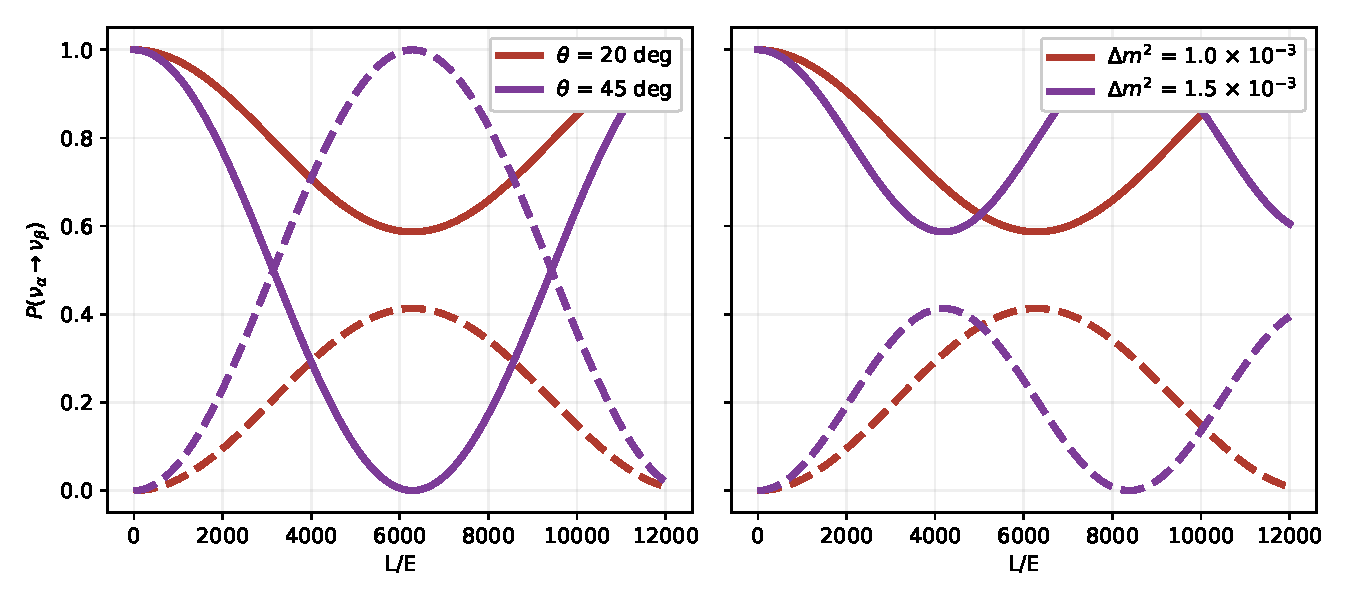
\includegraphics[width=0.9 \linewidth]{twoflavor.pdf}
\label{fig:twoflavor_probs}
\caption{The oscillation probabilities for survival (solid) and disappearance (dotted) in the two flavor regime. Left: Effect of changing the mixing angle while keeping the mass splitting at $10^-3$. Right: Effect of changing the mass splitting while fixing the mixing angle to 30 degrees.}
\end{figure}

The survival and disappearance probabilities are shown in Figure~\ref{fig:twoflavor_probs}.
As expected, changing the mixing angle directly affects the amplitude of the oscillations.
The characteristic $\texttt{L/E}$ scale is set by the mass splitting.
In the two flavor regime, the survival and disappearance probabilities sum to unity.
There is no dependence on the absolute mass scale or on the octant of the mixing angle.

For many experiments, careful planning may lead to the two flavor mixing being a reasonable approximation to the overall oscillation probability.


\label{subsec:msw}
\subsection{Matter Effects in Oscillation}
Calculations up to this point have assumed neutrinos oscilating in vacuum.
The effects of matter may be derived for the case of two neutrinos as well.
The modifications required for a description of matter effects begin with a modification of the Hamiltonian with a potential, $\mathtt{V}$, due to additional interactions during propagation.

\begin{equation}
H = H_0 + V
\end{equation}

The value of $\mathtt{H_0}$ is the value of vacuum Hamiltonian and can be shown \cite{Review-PMNS} to be

\begin{equation}
H_0 = \frac{\Delta m^2}{4E}
\begin{pmatrix}
- 2 \cos 2 \theta & \sin 2 \theta \\
\sin 2 \theta & 0 \\
\end{pmatrix}
\end{equation}

The new potential is produced by coherent forward scattering of neutrino on electrons and nucleons in the medium.
If this effect leaves the neutrino momentum unchanged, the resulting additional terms in the Hamiltonian may interfere with the propagation of the unscattered neutrinos.
The potential includes contributions from both charged-current and neutral-current interactions, although the charged-current interactions arise solely from the electron neutrinos.
The potential, expressed in the flavor basis, is then

\begin{equation}
V_{CC,\alpha} = 
\begin{cases}
\sqrt{2} \pm G_F n_e \left( x\right) & \alpha = e \\
0 & \alpha = \mu, \tau
\end{cases}\ \ \ \ \ 
V_{NC,\alpha} = -\frac{G_F}{\sqrt{2}} n_e\left(x\right)\;\;\; \alpha = e, \mu, \tau
\end{equation}

where a + is used for neutrinos and a - is used for antineutrinos.
The density of electrons, $n_e$ is a property of the medium while the value of $G_F$ is the Fermi coupling constant.
Note that the angle included here is that of the PMNS matrix in two diemsions.
The total Hamiltonian may be diagonalized by introducing $\theta_m$, an effective mixing angle in matter.

\begin{equation}
H = U_m 
\begin{pmatrix}
E_1^m & 0 \\
0 & E_2^m \\
\end{pmatrix}
U_m^\dagger \ \ \ \ \ 
U_m = \begin{pmatrix}
\cos \theta_m & \sin \theta_m \\
-\sin \theta_m & \cos \theta_m \\
\end{pmatrix}
\end{equation}

A number of quantities have here been introduced. 
A resonance density, known as the \emph{MSW resonance} for the names of theorists, Mikheyev, Smirnov, and Wolfenstein, who first proposed the effect
This density is defined by 

\begin{equation}
n_{res} = \frac{\Delta m^2 \cos 2 \theta}{2 \sqrt{2} G_F E}
\end{equation}

The resonant density is used to simplify the form of the matter energy states and mixing angles

\begin{equation}
E_2^m - E_1^m = \frac{\Delta m^2}{2 E} \sqrt{\left(1 \mp \frac{n_e}{n_{res}}\right)^2 \cos^2 2 \theta + \sin^2 2 \theta}
\end{equation}
\begin{equation}
\sin 2 \theta_m = \frac{\sin 2 \theta}{\left(1 \mp \frac{n_e}{n_{res}}\right)^2 \cos^2 2 \theta + \sin^2 2 \theta}
\end{equation}

where the negative sign is used for neutrinos and positive for antineutrinos.
The matter angle reaches maximal when $n_e = n_{res}$, at which point the oscillations are said to be at resonance.
This resonance occurs regardless of the standard oscillation mixing angle, although the mixing angle sets the overall scale of matter oscillations just as it does for vacuum oscillations.

In the case of constant matter densities, the oscillation probabilities in matter are then found straightforwadly in a manner identical to the vacuum case.
The disapperance probability is given by

\begin{equation}
P_m \left( \nu_\alpha \rightarrow \nu_\beta \right) = \sin^2 2 \theta_m \sin^2 \frac{\left( E_2^m - E_1^m\right) t}{2} \ \ \ \alpha \neq \beta
\label{eqn:twoflavor_msw}
\end{equation}

Here it becomes clear that the oscillation probabilities in matter follow the same form as Equation~\ref{eqn:two_flavor_disappearance}, but with an effect mixing angle $\theta_m$ and energy states $E_i^m$ set by the electron density of the medium.

Similar derivations may be performed using the full three-flavor framework. 
A full description of three flavor neutrino oscillation in the presence of a matter potential is beyond the scope of this work.
Further information and explicit forms may be found in \cite{Barger-Oscillations, Review-PMNS}.
In practice, many experiments are adequately described in the two-flavor framework described here.

